\documentclass[landscape]{standalone}

\usepackage{tikz}
\usepackage{pgf-umlcd}

\begin{document}

% Lens.h:class PixMapLens : public SampledLens {


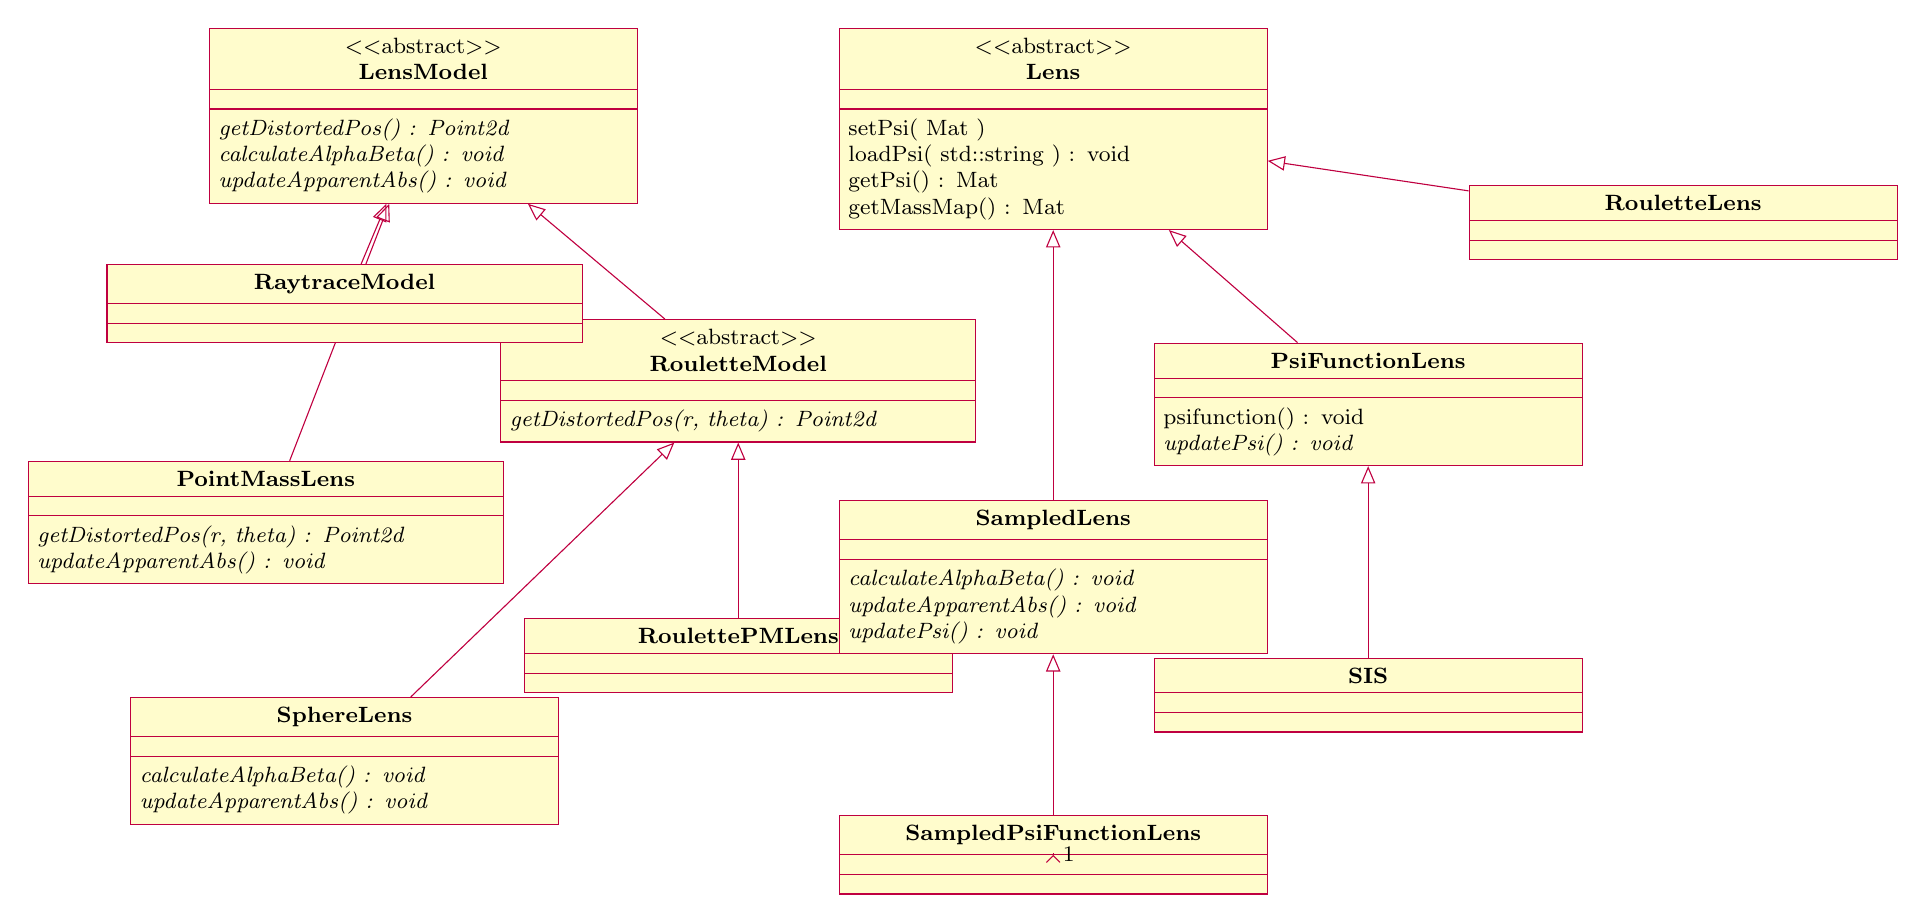
\begin{tikzpicture}
       \tikzstyle{every node}=[font=\footnotesize]

% Simulator.h:class LensModel {
   \begin{abstractclass}[text width = 52mm]{LensModel}{1 , 0}
      \operation[0]{getDistortedPos() : Point2d}
      \operation[0]{calculateAlphaBeta() : void}
      \operation[0]{updateApparentAbs()  : void}
   \end{abstractclass}

% Lens.h:class Lens {
   \begin{abstractclass}[text width = 52mm]{Lens}{9 , 0}
      \operation{setPsi( Mat )}
      \operation{loadPsi( std::string ) : void}
      \operation{getPsi() : Mat}
      \operation{getMassMap() : Mat}
   \end{abstractclass}

% Roulette.h:class RouletteModel : public LensModel { 
   \begin{abstractclass}[text width = 58mm]{RouletteModel}{5 , -3.7}
      \inherit{LensModel}
      \operation[0]{getDistortedPos(r, theta) : Point2d}
      % \operation[0]{markMask( InputOutputArray )}
      % \operation[0]{maskImage( InputOutputArray )}
      % \operation[0]{getMaskRadius() : double}
   \end{abstractclass}


% Simulator.h:class RaytraceModel : public LensModel { 
   \begin{class}[text width = 58mm]{RaytraceModel}{0 , -3}
      \inherit{LensModel}
   \end{class}

% Simulator.h:class PointMassLens : public LensModel { 
   \begin{class}[text width = 58mm]{PointMassLens}{-1 , -5.5}
      \inherit{LensModel}
      \operation[0]{getDistortedPos(r, theta) : Point2d}
      \operation[0]{updateApparentAbs()  : void}
   \end{class}

% Roulette.h:class SphereLens : public RouletteModel { 
   \begin{class}[text width = 52mm]{SphereLens}{0 , -8.5}
      \inherit{RouletteModel}
      % \operation{initAlphaBeta() : void}
      \operation[0]{calculateAlphaBeta() : void}
      \operation[0]{updateApparentAbs()  : void}
   \end{class}

% Roulette.h:class RoulettePMLens : public RouletteModel { 
   \begin{class}[text width = 52mm]{RoulettePMLens}{5 , -7.5}
      \inherit{RouletteModel}
      % \operation{initAlphaBeta() : void}
   \end{class}

% Lens.h:class SampledLens : public Lens {
   \begin{class}[text width = 52mm]{SampledLens}{9 , -6}
      \inherit{Lens}
      \operation[0]{calculateAlphaBeta() : void}
      \operation[0]{updateApparentAbs()  : void}
      \operation[0]{updatePsi()  : void}
   \end{class}

% Lens.h:class PsiFunctionLens : public Lens {
   \begin{class}[text width = 52mm]{PsiFunctionLens}{13 , -4}
      \inherit{Lens}
      \operation{psifunction() : void}
      \operation[0]{updatePsi()  : void}
   \end{class}

% Lens.h:class SampledPsiFunctionLens : public SampledLens {
   \begin{class}[text width = 52mm]{SampledPsiFunctionLens}{9 , -10}
      \inherit{SampledLens}
   \end{class}
   \unidirectionalAssociation{SampledPsiFunctionLens}{}{1}{SampledPsiFunctionLens}

% Lens.h:class RouletteLens : public Lens {
   \begin{class}[text width = 52mm]{RouletteLens}{17 , -2}
      \inherit{Lens}
   \end{class}

% Lens.h:class SIS : public PsiFunctionLens { 
   \begin{class}[text width = 52mm]{SIS}{13 , -8}
      \inherit{PsiFunctionLens}
   \end{class}
\end{tikzpicture}

\end{document}
